\chapter{References}
\setcounter{figure}{0}
\setcounter{table}{0}

\label{sec:References}

\section{Example Files}
\label{sec:ExampleFiles}
 The following examples are installed with OptimumTire.
 
 \begin{itemize}
\item	OptimumTire Add-in Example
\item	Matlab Examples
\item	OptimumTire Demo Project
\item	Custom Model Example Project
\end{itemize}

These files are installed with OptimumTire in the users documents folder under \textsl{OptimumTire Samples}

\section{Coordinate Systems}
\label{sec:CoordinateSystems}

OptimumTire allows the user to select between four different coordinate systems:

\begin{itemize}
\item	Society of Automotive Engineers (SAE) J670e
\item	Adapted SAE 
\item	International Organization for Standardization (ISO)
\item	Adapted ISO
\end{itemize}

Figure~\ref{fig:CoordinateSystems} shows the orientation of these coordinate systems and Figure~\ref{fig:ExampleCoordGraphs} shows graphs of typical tire parameters in the different coordinate systems.

\begin{figure}[H]
	\centering
		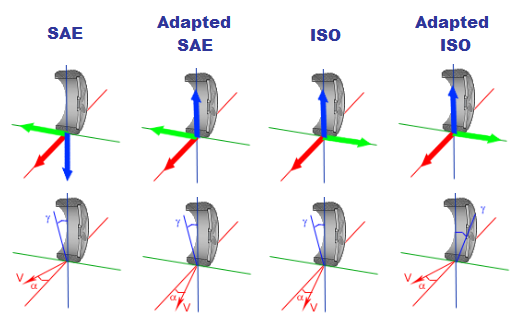
\includegraphics[width=1.0\textwidth]{CoordinateSystems.png}
	\caption{Coordinate Systems (viewed from front)}
	\label{fig:CoordinateSystems}
\end{figure}

\begin{figure}[H]
	\centering
		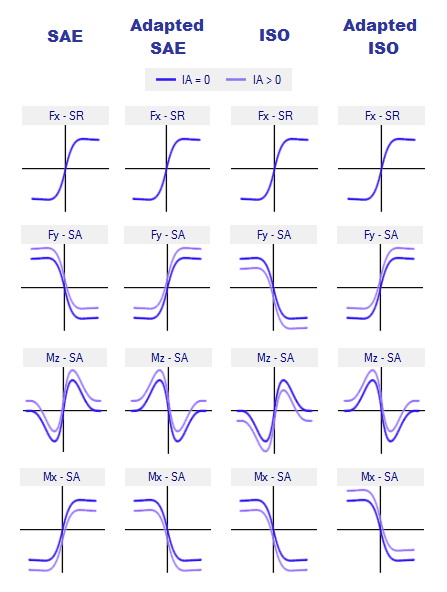
\includegraphics[width=1.0\textwidth]{ExampleCoordGraphs.png}
	\caption{Common Tire Parameters in different Coordinate Systems}
	\label{fig:ExampleCoordGraphs}
\end{figure}

\section{Units}
\label{sec:Units}
OptimumTire allows the user to select the units to be displayed. A summary of the available units are included in Table \ref{tbl:UnitsInOptimumT}.

\begin{table}[H]
	\centering
			\begin{tabular}{|c|c|c|c|c|}
			\hline
			\multicolumn{5}{|c|}{\cellcolor{tblue}\textbf{Units in OptimumTire}} \\ \hline
			\rowcolor{ttblue}Unit Type	& Angle	&Force	&Force / Angle & Force/Ratio	\\ \hline
			\multirow{8}{*}{Units}&	degree&	Newton & Newton/Degree&Newton	\\ \cline{2-5}
			&radian	&kilonewton	&Newton / radian&Newton / percent	 \\ \cline{2-5}
			& &	kilogram-force&	kilonewton / degree&	kilonewton \\ \cline{2-5}
			& & pound	&kilonewton / radian	&kilonewton / percent\\ \cline{2-5}
			& & & kilogram-force / degree  &	kilogram-force \\ \cline{2-5}
			& & & kilogram-force / radian  &	kilogram-force / percent \\ \cline{2-5}
			& & & pound / degree  &	pound \\ \cline{2-5}
			& & & pound / radian  &pound / percent \\ \hline
			
		\end{tabular}
		\caption{Units in OptimumTire}
		
\end{table}

\begin{table}[h]
	\centering
			\begin{tabular}{|c|c|c|c|c|}
			\hline
			\multicolumn{5}{|c|}{\cellcolor{tblue}\textbf{Units in OptimumTire}} \\ \hline
			\rowcolor{ttblue}Unit Type	& length & Moment	& Pressure	& Ratio	\\ \hline
			\multirow{6}{*}{Units} & meter & Newton meter	& bar &	Unit-less	\\ \cline{2-5}
			& centimeter & Newton millimeter &	Pascal & percent\\ \cline{2-5}
			& millimeter & kilonewton meter	& kilopascal	& \\ \cline{2-5}
			&	foot & kilogram-force meter	& pound / square inch & \\ \cline{2-5}
			&	mile & foot pound & & \\ \cline{2-5}
			& & inch pound & & \\ \hline
			
		\end{tabular}
		\caption{Units in OptimumTire}
		
\end{table}

\begin{table}[h]
	\centering
			\begin{tabular}{|c|c|c|c|}
			\hline
			\multicolumn{4}{|c|}{\cellcolor{tblue}\textbf{Units in OptimumTire}} \\ \hline
			\rowcolor{ttblue}Unit Type	&Stiffness	&Time& Velocity \\ \hline
			\multirow{8}{*}{Units}&Newton / meter	&second	&meter / second \\ \cline{2-4}
			&Newton / millimeter	&hour	&kilometer / hour\\ \cline{2-4}
			&kilonewton / meter	&&	feet / second\\ \cline{2-4}
			&kilonewton / millimeter	&&	mile / hour\\ \cline{2-4}
			&kilogram-force / meter		&&\\ \cline{2-4}
			&kilogram-force / millimeter	&&	\\ \cline{2-4}
			&pound / foot		&&\\ \cline{2-4}
			&pound / inch		&&\\ \hline

		\end{tabular}
	\caption{Units in OptimumTire}
	\label{tbl:UnitsInOptimumT}
\end{table}

\section{Fiala Model}
\label{sec:Fiala}
The Fiala tire model is based on the physical characteristics of the tire. Table \ref{tbl:FialaModelParameters} summarizes these characteristics. This model does not include combined longitudinal or lateral force, the effect of inclination angle, the lateral force offset at zero slip (from tire conicity or ply steer), or tire load sensitivity. More information about the Fiala model can be found in "The Multibody Systems Approach to Vehicle Dynamics", 2004, by Mike Blundell and Damian Harty.

\begin{table}[H]
	\centering
			\begin{tabular}{|c|c|c|}
			\hline
			\rowcolor{tblue}\multicolumn{2}{|c|}{\cellcolor{tblue}\textbf{Fiala Model Parameters}}&Unit Type \\ \hline
			R1 &	Tire tread width divided by two	&length \\ \hline
			Cs&	Longitudinal tire slip stiffness 	&force / ratio \\ \hline
			Calpha&	Lateral tire slip stiffness 	&force / angle \\ \hline
			Cr&	Rolling resistance moment coefficient 	&length \\ \hline
			U0&	Tire static friction coefficient	&ratio \\ \hline
			U1&	Tire sliding friction coefficient	&ratio \\ \hline
			\end{tabular}
	\caption{Fiala Model Parameters}
	\label{tbl:FialaModelParameters}
\end{table}

\section{Harty Model}
\label{sec:HartyModel}
The Harty tire model aims to provide a compromise between the complex Pacejka models and the limited Fiala model. Features of the Harty model include the ability to model camber thrust and the load dependency of cornering stiffness.

The model does not include the calculation of the overturning moment. The model also treats driving and braking forces as symmetric. Note the Harty model is only compatible with the SAE coordinate systems due to the method used to model the camber thrust. The model may still be graphed in other coordinate systems after fitting. For more information on the Harty model see "Intermediate tyre model for vehicle handling simulation" by M V Blundell and D Harty.

\subsubsection*{Longitudinal Model}

\begin{displaymath}
D= D_{x}+(|F_{z}|-R_{L})\frac{dD}{dF_{z}}
\end{displaymath}

\begin{displaymath}if( S < S_{c})\end{displaymath}
\begin{displaymath}
F_{x} = (1-e^{(-A_{x}|S/S_{c}|)})\mu DF_{z} sign(1,\alpha) 
\end{displaymath}

\begin{displaymath}if( S < S_{c})\end{displaymath}
\begin{displaymath}
F_{x} = (1-e^{-A_{x}})\mu DF_{z} sign(1,\alpha) 
\end{displaymath}

\subsubsection*{Lateral Model}

\begin{displaymath}
B= B_{y}+(|F_{z}|-R_{L})\frac{dB}{dF_{z}}
\end{displaymath}

\begin{displaymath}if( \alpha < \alpha_{c})\end{displaymath}
\begin{displaymath}
F_{y\alpha} = (1-e^{(-A_{y}|\alpha/\alpha_{c}|)})\mu BF_{z} sign(1,\alpha) 
\end{displaymath}

\begin{displaymath}if( \alpha > \alpha_{c})\end{displaymath}
\begin{displaymath}
F_{y\alpha} = (1-e^{-A_{y}})\mu BF_{z} sign(1,\alpha) 
\end{displaymath}

\begin{displaymath}
F_{y\gamma}=-F_{z}tan(\gamma)
\end{displaymath}

\begin{displaymath}
F_{y}=-F_{y\alpha}+F_{y\gamma}
\end{displaymath}

\subsubsection*{Aligning Torque Model}

\begin{displaymath}
C=C_{tz}+(|F_{z}|-R_{L})\frac{dC}{dF_{z}}
\end{displaymath}

\begin{displaymath}
L_{CP}=2(R_{1}^{2}-(\frac{R_{1}+F_{zk}}{K_{z}})^{2})^{0.5}
\end{displaymath}

\begin{displaymath}
x_{pt}=\frac{L_{CP}}{4}
\end{displaymath}

\begin{displaymath}if( \alpha < \alpha_{c})\end{displaymath}
\begin{displaymath}
M_{z}=-F_{y\alpha}Cx_{pt}(1-|\frac{\alpha}{\alpha_{c}}|)
\end{displaymath}

\begin{displaymath}if( \alpha > \alpha_{c})\end{displaymath}
\begin{displaymath}
M_{z}=0
\end{displaymath}

\subsubsection*{Rolling Resistance Model}

\begin{displaymath}if( V > 0)\end{displaymath}
\begin{displaymath}
M_{y}=-C_{r}F_{z}
\end{displaymath}

\begin{displaymath}if( V < 0)\end{displaymath}
\begin{displaymath}
M_{y}=C_{r}F_{z}
\end{displaymath}

The Harty model requires 14 parameters to model the tire.

\begin{table}[H]
\centering
\begin{tabular}{|c|l|c|}
		\hline
		\rowcolor{tblue}\multicolumn{2}{|c|}{\cellcolor{tblue}\textbf{Harty Model Parameters}}& Unit Type\\ \hline
		$F_{z0}$	& Reference tire load & force \\ \hline
		$R1$	&	Tire loaded radius & length \\ \hline
		$\alpha_c$	&		Critical slip angle & angle \\ \hline
		$A_y$	&	Curvature factor for lateral force  & \\ \hline
		$B_y$	&	Scale factor for lateral force at reference tire load & \\ \hline
		$dB/F_z$ &	Dimunition of lateral force scale factor with load & \\ \hline
		$S_c$	&	Critical slip ratio & ratio \\ \hline
		$A_x$	&	Curvature factor for longitudinal force & \\ \hline
		$C_{tz}$	&	Scale factor for aligning moment at reference tire load & \\ \hline
		$dC/F_z$ &	Dimunition of aligning moment scale factor with load & \\ \hline
		$D_x$	&	Scale factor for longitudinal force at reference tire load & \\ \hline
		$dD/F_z$ &	Dimunition of longitudinal force scale factor with load & \\ \hline
		$K_z$ & Tire vertical stiffness & force / length \\ \hline
		$C_r$ & Rolling resistance coefficient & length \\ \hline
		
		\end{tabular}
	\caption{Harty Model Parameters}
	\label{tbl:HartyModelParameters}
\end{table}

\section{Brush Model}
\label{sec:BrushModel}
Brush tire models can be very simple or very complex. The model included in OptimumTire is a very simple example of the brush model. The brush model is a physically based model that represents the tire as a row of elastic bristles that can deflect in the direction of the road. The deformation of these elements to applied forces represents the combined elasticity of the tire belt, carcass, and tread.

The model included in OptimumTire does not include the effects of inclination angle, the lateral force offset at zero slip (from tire conicity or ply steer), tire load sensitivity, or the fall off of force after the optimum slip has been reached. However, it does include the effects of combined lateral and longitudinal slip. 

\begin{table}[H]
	\centering
			\begin{tabular}{|c|c|c|}
			\hline
			\rowcolor{tblue}\multicolumn{2}{|c|}{\cellcolor{tblue}\textbf{Brush Model Parameters}}&Unit Type \\ \hline
				Fz0	&Nominal vertical load	&force\\ \hline
				mu	&Coefficient of friction	&ratio\\ \hline
				cpy	&Lateral tread element stiffness	&force / length\\ \hline
				cpx	&Longitudinal tread element stiffness &	force / length\\ \hline
				a0	&Contact patch length at Fz0 divided by two&	ratio\\ \hline
			\end{tabular}
	\caption{Brush Model Parameters}
	\label{tbl:BrushModelParameters}
\end{table}

\section{Pacejka Models}
\label{sec:PacejkaModels}
The Pacejka "Magic Formula" tire models are empirical relations that model the steady-state forces and moments produced by the tire as a function of the tire conditions (i.e. slip angle, slip ratio, inclination angle, etc �). These models include combined longitudinal and lateral force effects, inclination angle effects, lateral and longitudinal force offset, and tire load sensitivity. The primary form for the Pacejka models is given in the equations below. The table following these equations describes the various parameters.

\begin{displaymath}
y=D\sin\left[C\arctan\left\{Bx-E\left(Bx-\arctan{Bx}\right)\right\}\right]
\end{displaymath}
With
\begin{displaymath}
Y(X)= y(x)+ S_V
\end{displaymath}
\begin{displaymath}
x=X+S_H
\end{displaymath}

\begin{table}[H]
	\centering
			\begin{tabular}{|c|c|c|}
			\hline
			\multicolumn{3}{|c|}{\cellcolor{tblue}\textbf{General Pacejka Parameters}} \\ \hline
			\rowcolor{ttblue}\multicolumn{2}{|c|}{\cellcolor{ttblue}\textbf{Input/Output}}&Description \\ \hline
			Y	&Output	&Lateral force, longitudinal force, or aligning torque \\ \hline
			X	&Input	&Slip ratio or tangent of slip angle \\ \hline
			\rowcolor{ttblue}\multicolumn{2}{|c|}{\cellcolor{ttblue}\textbf{Parameters}}&Description \\ \hline
			B	&Stiffness Factor	&Slope at the origin \\ \hline
			C	&Shape Factor	&Shape of the resulting curve \\ \hline
			D	&Peak Value	&Peak Value with C>=1 \\ \hline
			E	&Curvature Factor	&Curvature and horizontal position of the peak \\ \hline
			H	&Horizontal Shift	& \\ \hline
			V	&Vertical Shift	& \\ \hline
			\end{tabular}
	\caption{Pacejka Model}
	\label{tbl:PacejkaModel}
\end{table}

A description of the Pacejka models implemented in OptimumTire is given in this section. In the following section the coefficients used in these models are summarized.

\subsection{Pacejka '96}
\label{sec:Pacejka96}
This model is given in the 1996 paper "The Tire as a Vehicle Component" by Hans B. Pacejka. This model includes the combined lateral and longitudinal tire response as well as lateral camber response and load sensitivity. This model does not include the rolling resistance or overturning moment of the tire. This model includes 78 coefficients.

\subsection{Pacejka 2002}
\label{sec:Pacejka2002}
 This model is given in Pacejka's book "Tire and Vehicle Dynamics" published in 2002. It is similar to the '96 model but has additional coefficients in the combined lateral and longitudinal models. It also includes models for the rolling resistance and overturning moment. This model includes 89 coefficients.

\subsection{Pacejka 2002 with Inflation Pressure Effects}
\label{sec:Pacejka2002withInflationPressureEffects}
This model is described in the paper "Extending the Magic Formula and SWIFT Tyre Models for Inflation Pressure Changes" by Dr. Ir. A.J.C. Schmeitz, Dr. Ir. I.J.M. Besselink, Ir. J. de Hoogh, and Dr. H. Nijmeijer. This model incorporates the effect of inflation pressure into the Pacejka 2002 model. Ten additional coefficients, including the reference pressure Pi0, are added to the model. These coefficients appear in the pure lateral, longitudinal, and aligning torque models. This model includes 99 coefficients.

\subsection{Magic Formula 5.2}
\label{sec:MagicFormula52}
This model is a close development of the the Pacejka 2002 model. This model differs from Pacejka 2002 in the way that it models the effect of camber. The main advantage of the MF5.2 model is that models the effect of camber on the longitudinal coefficient of friction. This model includes 90 coefficients.

\subsection{Magic Formula 6.1}
\label{sec:MagicFormula61}
This model is a further development of the the Magic Formula 5.2 model. This model improves the description of camber, allowing the model to handle a very large range of camber angles. This makes special "`special"' motorcycle Magica Formula superfluous. In addition the model also allows for better modelling of inflation pressure changes and rolling resistance. For most tires the Magic Formula 6.1 will give slightly better results compared to Magic Formula 5.2. This model includes 155 coefficients.

\subsection{Pacejka 2006}
\label{sec:Pacejka2006}
This model is given in the second edition of Pacejka's book "Tire and Vehicle Dynamics" published in 2006. This model is based off of the 2002 model but includes significant modifications to the pure lateral and aligning torque models. An additional coefficient is also added to both the combined lateral and longitudinal models. This model includes 97 coefficients.

\section{Pacejka Coefficients}
\label{sec:PacejkaCoefficients}
Table~\ref{tbl:PacejkaCoefficents} displays all of the Pacejka coefficients used in OptimumTire. These coefficients are grouped into nine different categories depending on what tire characteristics they describe: General, Pure Lateral, Pure Longitudinal, Aligning Torque, Combined Lateral, Combined Longitudinal, Combined Aligning Torque, Overturning Moment and Rolling Resistance. 
On the left the name and a brief description of the coefficient are given. On the right the "x" in the boxes indicates whether or not each coefficient is included in each of the specific Pacejka models.

\begin{center}
\begin{longtable}[c]{|c|p{4in}|cccc|}
\hline
			\rowcolor{tblue}\multicolumn{2}{c}{\cellcolor{tblue}\textbf{Pacejka Coefficents}}&\multicolumn{4}{c}{\cellcolor{tblue}\textbf{Models}}\\\hline
			
			\rowcolor{ttblue}\multicolumn{2}{c}{\cellcolor{ttblue}\textbf{General}}&96&02&02Pi&06\\\hline
			
			Fz0	&Nominal load &x&x&x&x\\ \hline
			r0	&Tire unloaded radius	&x&x&x&x\\ \hline
			V0	&Reference velocity &&x&x&x\\ \hline
			Pi0	&Reference pressure &&&x&\\ \hline
%			&&&&& \\ \hline
			\rowcolor{ttblue}\multicolumn{2}{|c|}{\cellcolor{ttblue}\textbf{Pure Lateral}}&96&	02& 	02Pi&06\\ \hline
			pCy1	&Shape factor	&x	&x 	&x	&x\\ \hline
			pDy1	&Lateral coefficient of friction at Fz0	&x &x		&x	&x\\ \hline
			pDy2	&Variation of friction with load	&x	&x &x		&x\\ \hline
			pDy3	&Variation of friction with camber squared	&x 	&x	&x	&x\\ \hline
			pEy1	&Lateral curvature at Fz0	&x	&x 	&x	&x\\ \hline
			pEy2	&Variation of curvature with load	&x	&x	&x	&x\\ \hline
			pEy3	&Zero order camber dependency of curvature	&x &x		&x	&x\\ \hline
			pEy4	&Variation of curvature with camber	&x	&x	&x	&x\\ \hline
			pEy5	&Camber curvature				&&&&x\\ \hline
			pKy1	&Maximum cornering stiffness	&x	&x &x		&x\\ \hline
			pKy2	&Load at which maximum stiffness occurs	&x &x		&x	&x\\ \hline
			pKy3	&Variation of stiffness with camber	&x	&x	&x	&x\\ \hline
			pKy4	&Variation of stiffness with camber squared		&&&&x\\ \hline
			pKy5	&Lateral stiffness dependency with camber				&&&&x\\ \hline
			pKy6	&Camber stiffness factor				&&&&x\\ \hline
			pKy7	&Load dependency of camber stiffness factor				&&&&x\\ \hline
			pHy1	&Horizontal shift at Fz0	&x	&x &x	&x\\ \hline
			pHy2	&Variation of horizontal shift with load	&x &x	&x	&x\\ \hline
			pHy3	&Variation of horizontal shift with camber	&x &x		&x	&\\ \hline
			pVy1	&Vertical shift at Fz0	&x &x		&x	&x\\ \hline
			pVy2	&Variation of vertical shift with load	&x	&x 	&x	&x\\ \hline
			pVy3	&Variation of vertical shift with camber	&x	&x 	&x	&x\\ \hline
			pVy4	&Variation of vertical shift with camber and load 	&x 	&x	&x	&x\\ \hline
			pPy1	&Variation of cornering stiffness with inflation pressure			&&&x&	\\ \hline
			pPy2	&Variation of cornering stiffness with inflation and load	&&&x&	\\ \hline
			pPy3	&Variation of friction with inflation pressure 			&&&x&	\\ \hline
			pPy4	&Variation of friction with inflation pressure squared	&&&x&	\\ \hline
%			&&&&& \\ \hline
			\rowcolor{ttblue}\multicolumn{2}{|c|}{\cellcolor{ttblue}\textbf{Pure Longitudinal}}&96&	02&	 02Pi&	06 \\ \hline
			pCx1	&Shape factor	&x	&x		&x &x\\ \hline
			pDx1	&Longitudinal coefficient of friction at Fz0	&x &x		&x	&x\\ \hline
			pDx2	&Variation of friction with load	&x	&x &x		&x\\ \hline
			pDx3	&Variation of friction with camber	&	& 	&	&\\ \hline
			pEx1	&Longitudinal curvature at Fz0	&x	&x 	&x	&x\\ \hline
			pEx2	&Variation of curvature with load	&x	&x &x		&x\\ \hline
			pEx3	&Variation of curvature with load squared 	&x &x		&x&	x\\ \hline
			pEx4	&Factor in curvature while driving 	&x	&x	&x 	&x\\ \hline
			pKx1	&Longitudinal slip stiffness at Fz0	&x	&x	&x	&x\\ \hline
			pKx2	&Variation of slip stiffness with load	&x	&x	&x	&x\\ \hline
			pKx3	&Exponent in slip stiffness with load	&x	&x 	&x	&x\\ \hline
			pHx1	&Horizontal shift at Fz0	&x	&x	&x	&x\\ \hline
			pHx2	&Variation of horizontal shift with load 	&x 	&x	&x	&x\\ \hline
			pVx1	&Vertical shift at Fz0	&x	&x 	&x	&x\\ \hline
			pVx2	&Variation of vertical shift with load	&x	&x &x	&x\\ \hline
			pPx1	&Variation of slip stiffness with inflation pressure 	&&&x&	\\ \hline
			pPx2	&Variation of slip stiffness with inflation pressure squared	&&&x&	\\ \hline
			pPx3	&Variation of friction with inflation pressure 			&&&x&	\\ \hline
			pPx4	&Variation of friction with inflation pressure squared	&&&x&	\\ \hline
%			&&&&& \\ \hline
			\rowcolor{ttblue}\multicolumn{2}{|c|}{\cellcolor{ttblue}\textbf{Aligning Torque}}&96&	02& 02Pi&	06 \\ \hline
			qBz1	&Pneumatic trail slope factor at Fz0	&x	&x 	&x	&x\\ \hline
			qBz2	&Variation of trail slope with load	&x	&x &x	&x\\ \hline
			qBz3	&Variation of trail slope with load squared	&x 	&x	&x	&x\\ \hline
			qBz4	&Variation of trail slope with camber	&&&&x		\\ \hline
			qBz5	&Variation of trail slope with  absolute camber	&x &x	&x	&x\\ \hline
			qBz6	&Variation of trail slope with camber squared		&&x	 &x	&x\\ \hline
			qBz9	&Slope factor of residual torque	&x	&x 	&x	&x\\ \hline
			qBz10	&Slope factor of residual torque	&x	&x	&x	&x\\ \hline
			qCz1	&Shape factor for pneumatic trail	&x	&x 	&x	&x\\ \hline
			qDz1	&Peak pneumatic trail	&x	&x 	&x	&x\\ \hline
			qDz2	&Variation of peak trail with load 	&x	&x &x		&x\\ \hline
			qDz3	&Variation of peak trail with  camber	&x	&x &x	&x\\ \hline
			qDz4	&Variation of peak trail with camber squared	&x &x		&x	&x\\ \hline
			qDz6	&Peak residual torque	&x	&x &x		&x\\ \hline
			qDz7	&Variation of peak torque with load	&x &x	&x		&x\\ \hline
			qDz8	&Variation of peak torque with camber	&x	&x &x		&x\\ \hline
			qDz9	&Variation of peak torque with camber and load	&x &x		&x	&x\\ \hline
			qDz10	&Variation of peak torque with camber squared			&&&&	x\\ \hline
			qDz11	&Variation of peak torque with camber squared and load 		&&&&x\\ \hline
			qEz1	&Pneumatic trail curvature at Fz0	&x	&x &x	&x\\ \hline
			qEz2	&Variation of curvature with load 	&x	&x &x	&x\\ \hline
			qEz3	&Variation of curvature with load squared	&x	&x &x	&x\\ \hline
			qEz4	&Variation of curvature with sign of slip angle    	&x &x	&x	&x\\ \hline
			qEz5	&Variation of curvature with camber and sign of slip angle  	&x &x	&x	&x\\ \hline
			qHz1	&Pneumatic trail horizontal shift at Fz0	&x	&x &x	&x\\ \hline
			qHz2	&Variation of horizontal shift with load	&x	&x &x	&x\\ \hline
			qHz3	&Variation of horizontal shift with camber	&x	&x &x	&x\\ \hline
			qHz4	&Variation of horizontal shift with camber and load	&x &x	&x	&x\\ \hline
			qPz1	&Variation of peak with inflation pressure			&&&x&	\\ \hline
%			&&&&& \\ \hline
			\rowcolor{ttblue}\multicolumn{2}{|c|}{\cellcolor{ttblue}\textbf{Combined Lateral}}&96&	02&	02Pi&	06 \\ \hline
			rBy1	&Slope factor for combined slip lateral force reduction	&x	&x &x		&x\\ \hline
			rBy2	&Variation of lateral force slope reduction with slip angle	&x	&x 	&x	&x\\ \hline
			rBy3	&Shift factor for slip angle in lateral force slope reduction	&x  &x  &x  &x\\ \hline
			rBy4	&Variation of lateral force combined stiffness with camber	&	&	&	&x\\ \hline
			rCy1	&Shape factor for combined slip lateral force reduction		&&x	&x	 &x\\ \hline
			rEy1	&Curvature factor of combined lateral force		&&x	&x 	&x\\ \hline
			rEy2	&Curvature factor of combined lateral force with load	&x	&x 	&x	&x\\ \hline
			rHy1	&Horizontal shift factor for lateral force reduction		&&x	 &x	&x\\ \hline
	 		rHy2	&Horizontal shift factor for lateral force reduction with load	&x	 &x	&x	&x\\ \hline
			rVy1	&Vertical shift at Fz0 for lateral force reduction 	&x	&x &x	&x\\ \hline
			rVy2	&Variation of vertical shift factor with load	&x	&x	&x &x\\ \hline
			rVy3	&Variation of vertical shift factor with camber	&x	&x	&x 	&x\\ \hline
			rVy4	&Variation of vertical shift factor with slip angle	&x	&x	&x	&x\\ \hline
			rVy5	&Variation of vertical shift factor with slip ratio	&x	&x 	&x	&x\\ \hline
			rVy6	&Variation of vertical shift factor with the arctan of slip ratio	&x &x	&x	&x\\ \hline
%			&&&&& \\ \hline
			\rowcolor{ttblue}\multicolumn{2}{|c|}{\cellcolor{ttblue}\textbf{Combined Longitudinal}}&96&	02&	02Pi&	06 \\ \hline
			rBx1	&Slope factor for combined slip longitudinal force reduction	&x	&x 	&x	&x\\ \hline
			rBx2	&Variation of longitudinal force slope reduction with slip ratio	&x 	&x	&x	&x\\ \hline
			rBx3	&Variation of longitudinal force combined stiffness with camber				&&&&x\\ \hline
			rCx1	&Shape factor for combined slip longitudinal force reduction	&x &x	&x	&x\\ \hline
			rEx1	&Curvature factor of combined longitudinal force		&&x	&x &x\\ \hline
			rEx2	&Curvature factor of combined longitudinal force with load		&&x	 &x &x\\ \hline
			rHx1	&Shift factor for combined slip longitudinal force reduction	&x	&x	&x	&x\\ \hline
%			&&&&& \\ \hline
			\rowcolor{ttblue}\multicolumn{2}{|c|}{\cellcolor{ttblue}\textbf{Combined Aligning Torque}}&96&	02& 	02Pi&	06 \\ \hline
			sSz1	&Effect of longitudinal force on aligning torque	&x	&x 	&x	&x\\ \hline
			sSz2	&Variation of aligning torque with lateral force	&x	&x 	&x	&x\\ \hline
			sSz3	&Variation of aligning torque with camber	&x	&x	&x &x	\\ \hline
			sSz4	&Variation of aligning torque with camber and load	&x &x		&x	&x\\ \hline
%			&&&&& \\ \hline
			\rowcolor{ttblue}\multicolumn{2}{|c|}{\cellcolor{ttblue}\textbf{Overturning Moment}}&96&	02& 02Pi&	06 \\ \hline
			qSx1	&Vertical force induced overturning moment		&&x	&x 	&x\\ \hline
			qSx2	&Camber induced overturning moment		&&x	&x 	&x\\ \hline
			qSx3	&Lateral force induced overturning moment		&&x	 &x	&x\\ \hline
%			&&&&& \\ \hline
			\rowcolor{ttblue}\multicolumn{2}{|c|}{\cellcolor{ttblue}\textbf{Rolling Moment}}&96&	02&	 02Pi&	06 \\ \hline
			qSy1	&Rolling resistance torque coefficient		&&x	&x	&x \\ \hline
			qSy2	&Variation of rolling resistance torque with load		&&x	&x	&x \\ \hline
			\caption{Pacejka Coefficents}
			\label{tbl:PacejkaCoefficents}
\end{longtable}
\end{center}

\section{Pacejka Scaling Factors}
\label{sec:PacejkaScalingFactors}

Table~\ref{tbl:PacejkaScalingCoefficients} below gives a summary of the Pacejka scaling coefficients. The default value for all of these coefficients is 1 except for $\lambda\mu V$ which is 0.

\begin{center}
\begin{longtable}[c]{|c|p{4in}|cccc|}
	\hline
			
			\multicolumn{2}{|c|}{\cellcolor{tblue}\textbf{Scaling Factors}}&\multicolumn{4}{|c|}{\cellcolor{tblue}\textbf{Models}} \\ \hline
			\rowcolor{ttblue}\multicolumn{2}{|c|}{\cellcolor{ttblue}\textbf{Pure Slip}}&96&	02&	02Pi&	06 \\ \hline
			$\lambda F_{z0}$ &Nominal load factor	&x	&x	&x	&x\\ \hline
			$\lambda \mu x$	&Peak longitudinal coefficient of friction	&x	&x &x	&x\\ \hline
			$\lambda \mu y$	&Peak lateral coefficient of friction	&x	&x &x	&x\\ \hline
			$\lambda \mu V$	&Friction decay with slip speed 		&&x	&x &x\\ \hline
			$\lambda Kx\kappa$	&Longitudinal slip stiffness	&x	&x &x	&x\\ \hline
			$\lambda Ky \alpha$	&Cornering stiffness 	&x	&x &x	&x\\ \hline
			$\lambda Cx$	&Longitudinal shape factor	&x	&x &x	&x\\ \hline
			$\lambda Cy$	&Lateral shape factor	&x	&x	&x &x\\ \hline
			$\lambda Ex$	&Longitudinal curvature factor	&x &x	&x	&x\\ \hline
			$\lambda Ey$	&Lateral curvature factor	&x	&x	&x &x\\ \hline
			$\lambda Hx$	&Longitudinal horizontal shift 	&x	&x &x	&x\\ \hline
			$\lambda Hy$	&Lateral horizontal shift 	&x	&x	&x &x\\ \hline
			$\lambda Vx$	&Longitudinal vertical shift	&x	&x	&x	&x\\ \hline
			$\lambda Vy$	&Lateral vertical shift	&x	&x &x	&x	\\ \hline
			$\lambda Ky \gamma$	&Camber force stiffness 	&x	&x &x	&x\\ \hline
			$\lambda Kz \gamma$	&Camber torque stiffness 	&x	&x &x	&x\\ \hline
			$\lambda t$	&Pneumatic trail (effects aligning torque stiffness) 	&x &x	&x	&x\\ \hline
			$\lambda Mr$	&Residual torque 	&x	&x &x	&x\\ \hline
%			&&&&&\\ \hline
			\rowcolor{ttblue}\multicolumn{2}{|c|}{\cellcolor{ttblue}\textbf{Combined Slip}}&96&	02& 02Pi&	06 \\ \hline					
			$\lambda x \alpha$	&Slip angle influence on longitudinal force	&x	&x &x	&x\\ \hline
			$\lambda y \kappa$	&Slip ratio influence on lateral force 	&x	&x	&x &x\\ \hline
			$\lambda Vy \kappa$	&Slip ratio induced lateral force from ply steer 	&x &x	&x	&x\\ \hline
			$\lambda s$	&Aligning torque moment arm of longitudinal force 	&x	&x &x	&x\\ \hline
%			&&&&&\\ \hline
			\rowcolor{ttblue}\multicolumn{2}{|c|}{\cellcolor{ttblue}\textbf{Other}}&96&	02&	02Pi&	06 \\ \hline					
			$\lambda Cz \alpha$	&Radial tire stiffness	&	&x	&x &x\\ \hline
			$\lambda Mx \kappa$	&Overturning couple stiffness 	&	&x &x	&x\\ \hline
			$\lambda My \kappa$	&Rolling resistance moment	&	&x	&x &x\\ \hline
%			&&&&&\\ \hline
			\caption{Pacejka Scaling Coefficients}
			\label{tbl:PacejkaScalingCoefficients}
\end{longtable}
\end{center}
